\chapter{Concepts for the proposed system \\ 
% \small{\textit{-- Author Name}}
\index{Concepts for the proposed system}
\label{Chapter::Conceptsfortheproposedsystem}} 
\section{Background, objectives, and scope \label{Section::Backgroundobjectivesandscope}}
\begin{enumerate}
    
    \item Multi-store support: The system will support multiple stores, allowing store managers and staff to manage inventory across multiple locations. This will provide centralized inventory control and enable inventory transfers between stores.

    \item Mobile access: The system will provide mobile access, allowing store managers and staff to access inventory data and perform inventory management tasks from anywhere at any time. This will enable remote inventory management and reduce the need for physical presence in the store.

    \item Customizable alerts: The system will enable customizable alerts that notify store managers and staff of low inventory levels, stockouts, and other inventory-related issues. Alerts can be customized to specific thresholds and sent via email, SMS, or in-app notifications.

    \item Integration with POS system: The system will integrate with the point-of-sale (POS) system, allowing inventory levels to be automatically updated based on sales transactions. This will ensure accurate inventory tracking and reduce errors related to manual data entry.

    \item Vendor management: The system will include vendor management functionality, allowing store managers and staff to manage vendor relationships and track vendor performance. This will help optimize the purchasing process and ensure timely delivery of goods.

\end{enumerate}

\section{Operational policies and constraints \label{Section::Operationalpoliciesandconstraints}}
\textbf{Operational policies}:
\begin{enumerate}
    \item Access control: Access to the instore inventory management system will be restricted to authorized personnel only. Access credentials will be assigned on a need-to-know basis.

    \item Data protection: The system will store inventory data in a secure and encrypted manner. Data backups will be taken regularly to ensure data integrity and availability in case of system failure.

    \item Maintenance and support: The system will be maintained and supported by trained personnel to ensure optimal performance and reliability. Maintenance schedules will be developed to minimize disruptions to store operations.

    \item Training and documentation: Store managers and staff will be provided with adequate training and documentation to ensure proper use of the system. Training will be ongoing, and documentation will be updated as needed.

    \item Change management: Changes to the system, including upgrades and modifications, will be managed through a formal change management process. Changes will be tested and validated before implementation.
\end{enumerate}
\textbf{Constraints}:
\begin{enumerate}
    \item Budget: The implementation of the instore inventory management system will be subject to budgetary constraints. The cost of hardware, software, and personnel will need to be within the allocated budget.

    \item Integration with existing systems: The system will need to be integrated with the existing point-of-sale (POS) system, which may have limitations on compatibility.

    \item Technical limitations: The system will be subject to technical limitations, such as hardware availability and bandwidth limitations as the system may need to be operated in remote areas where connectivity is scarce.

    \item User adoption: The success of the system will depend on the adoption by store managers and staff. The system will need to be user-friendly and intuitive to ensure adoption.

    \item Regulatory compliance: The system will need to comply with all relevant regulatory requirements, including data privacy and security regulations.
\end{enumerate}
\section{Description of the proposed system \label{Section::Descriptionoftheproposedsystem}}

The proposed instore inventory management system is a web-based software solution designed to help retailers and store managers manage their inventory more efficiently and effectively. The system will include the following key features:

\begin{enumerate}
    \item Multi-store support: Supports multiple stores with centralized inventory control and transfers between stores.

    \item Mobile access: Provides mobile access for remote inventory management.

    \item Customizable alerts: Enables customizable alerts for low inventory levels and other inventory-related issues.

    \item Integration with POS system: Integrates with POS system for automatic inventory updates.

    \item Vendor management: Includes vendor management functionality for managing vendor relationships and tracking performance.

    \item Reporting and analytics: Provides real-time reporting and analytics for data-driven decision making.

    \item User roles and permissions: Has different user roles and permissions for authorized access and data security.

    \item Security and data privacy: Ensures security and privacy of inventory data and user information with robust security features.
\end{enumerate}
The proposed instore inventory management system will provide retailers and store managers with a comprehensive solution for managing their inventory more efficiently and effectively. It will enable centralized inventory control, remote inventory management, and real-time reporting and analytics to help optimize inventory management strategies and improve overall store performance.

\begin{figure}[H]
  \centering
   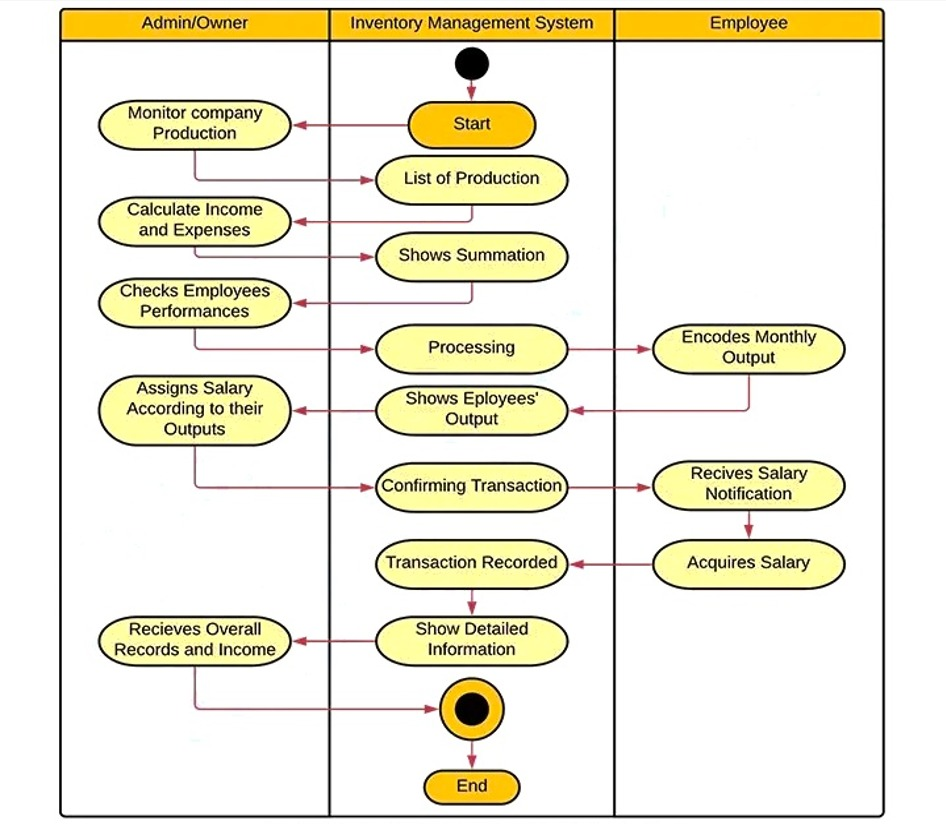
\includegraphics[width=9cm]{Figures/ActivityDiagram.jpeg}
  \caption{Activity Diagram of the system}
\label{}
\end{figure}

\begin{figure}[H]
  \centering
   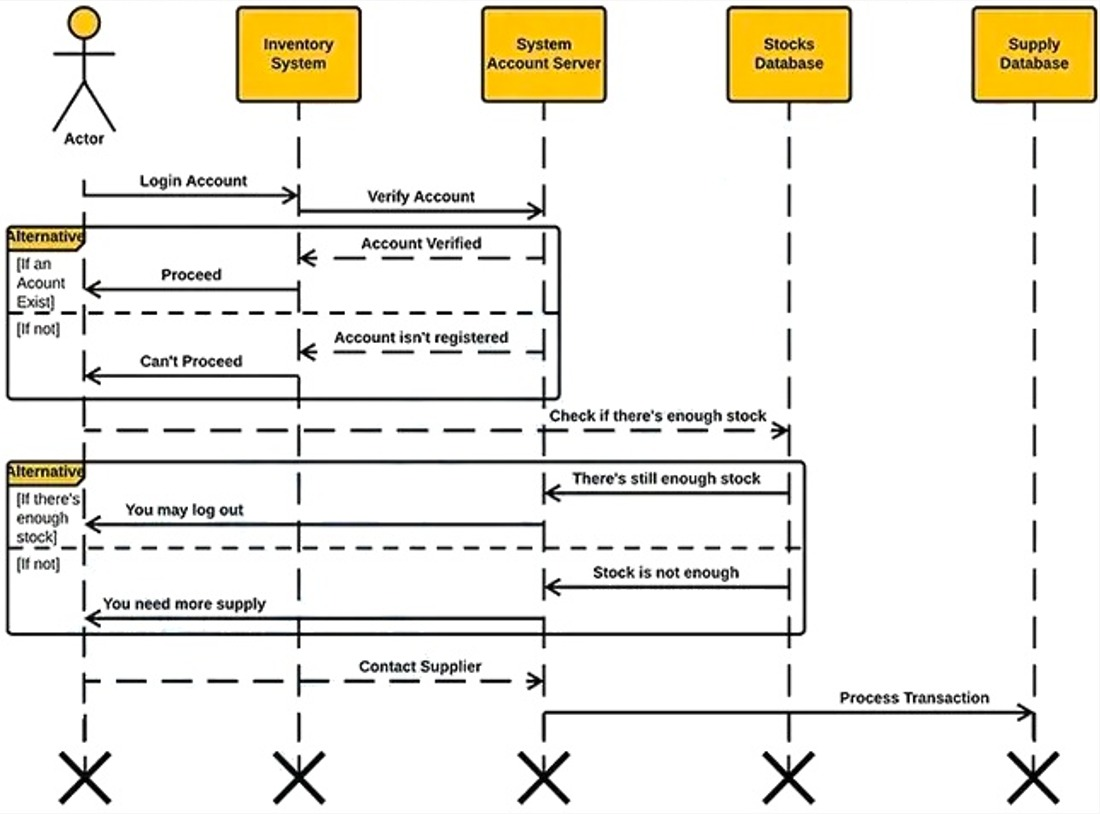
\includegraphics[width=9cm]{Figures/SequenceDiagram.jpeg}
  \caption{Sequence Diagram}
\label{}
\end{figure}

\section{Modes of operation \label{Section::Modesofoperation}}

\begin{enumerate}

    \item Online mode: Allows real-time access to inventory data through a web-based interface.

    \item Offline mode: Enables offline access to inventory data with local storage capabilities, and synchronization with the online system when an internet connection is available.

    \item Mobile mode: Provides mobile access to inventory data through a mobile application that is compatible with both Android and iOS devices.

    \item API mode: Allows integration with third-party systems through RESTful APIs for data sharing and system integration.

    \item Backup and recovery mode: Ensures data backup and recovery capabilities in case of system failures, data loss, or other disruptions.
\end{enumerate}

\section{User classes and other involved personnel \label{Section::Userclassesandotherinvolvedpersonnel}}
\begin{enumerate}
    \item Store managers: Responsible for managing inventory levels, overseeing stock movements, and making purchasing decisions.

    \item Sales staff: Responsible for tracking inventory movements, processing sales transactions, and updating inventory levels in real-time.

    \item Warehouse staff: Responsible for receiving and processing incoming shipments, managing inventory levels, and preparing outgoing shipments.

    \item IT staff: Responsible for system maintenance, upgrades, and technical support for the inventory management system.

    \item Auditors: Responsible for conducting periodic audits of inventory data and transactions to ensure accuracy and compliance with regulatory requirements.

    \item Vendors: Involved in the inventory management system as suppliers of goods and services, and can access the system for order management and delivery tracking.
\end{enumerate}
\begin{figure}[H]
  \centering
   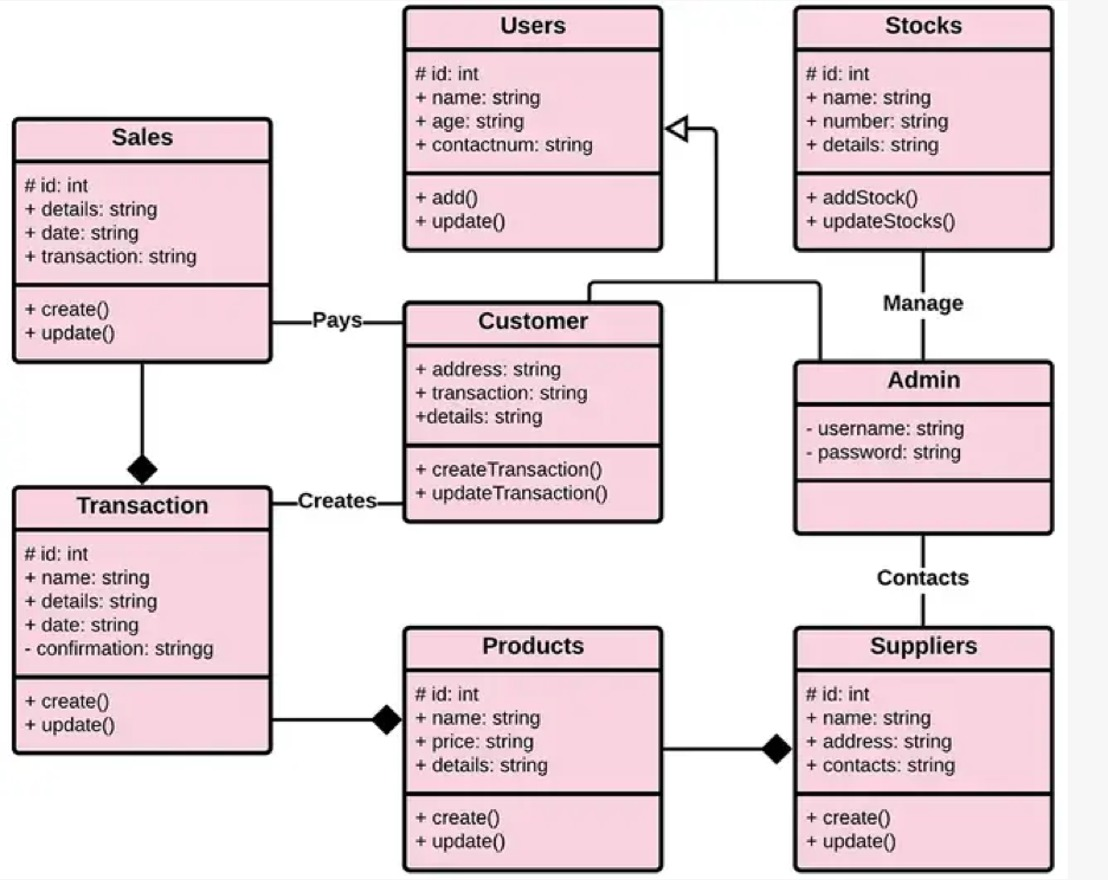
\includegraphics[width=9cm]{Figures/ClassDiagram.jpeg}
  \caption{Class Diagram of the proposed system}
\label{}
\end{figure}

\section{Support environment \label{Section::Supportenvironment}}

\begin{enumerate}
    \item Helpdesk and support services: A centralized helpdesk to provide technical support, assistance, and guidance to system users.

    \item Knowledge base and documentation: A comprehensive knowledge base and documentation system to provide users with resources and self-help tools to resolve issues and answer frequently asked questions.

    \item System maintenance and upgrades: Regular maintenance and upgrades of the system to ensure optimal performance, reliability, and security.

    \item Training and education: Training and education programs for users to ensure they have the necessary knowledge and skills to effectively use the system.

    \item User feedback and feature requests: A mechanism for users to provide feedback and suggest new features and enhancements to the system.
\end{enumerate}
\newpage